\documentclass{standalone}
\usepackage{tikz}
\usepackage{ctex,siunitx}
\setCJKmainfont{Noto Serif CJK SC}
\usepackage{tkz-euclide}
\usepackage{amsmath}
\usetikzlibrary{patterns, calc,3d}
\usetikzlibrary {decorations.pathmorphing,decorations.pathreplacing,decorations.shapes}
\begin{document}
\small
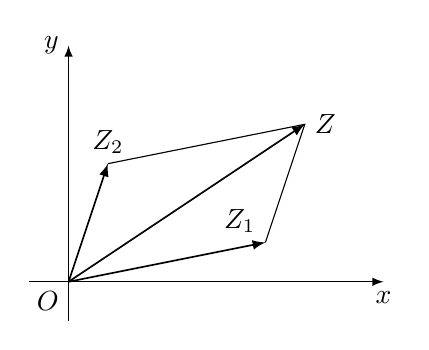
\begin{tikzpicture}[>=latex,scale=1.0]
  \draw[->](-0.5,0)--(4,0)node[below]{$x$};
  \draw[->](0,-0.5)--(0,3)node[left]{$y$};
  \node at (0,0)[below left]{$O$};
  \draw[semithick,->](0,0)--(2.5,0.5)node[above left]{$Z_1$};
  \draw[semithick,->](0,0)--(0.5,1.5)node[above]{$Z_2$};
  \draw[semithick,->](0,0)--(3,2)node[right]{$Z$};
  \draw(0.5,1.5)--(3,2)--(2.5,0.5);
\end{tikzpicture}
\end{document}